\usetikzlibrary{arrows.meta,decorations.pathreplacing}

\begin{frame}{address/page table entry format}

(with POBITS=12, LEVELS=1)
\small
\begin{tabular}{l|l|l|l|l}
    ~ & bits 63--21 & bits 20--12 & bits 11--1 & bit 0 \\ \hline
    page table entry & \multicolumn{2}{c|}{physical page number} & unused & valid bit \\ \hline
    virtual address & unused &virtual page number & \multicolumn{2}{c}{page offset} \\ \hline
    physical address & \multicolumn{2}{c|}{physical page number} & \multicolumn{2}{c}{page offset} \\ \hline
\end{tabular}
\begin{itemize}
\item in assignment: value from posix\_memalign = physical address
\end{itemize}
\end{frame}

\begin{frame}[plain]{pa = translate(va) [LEVELS=1]}
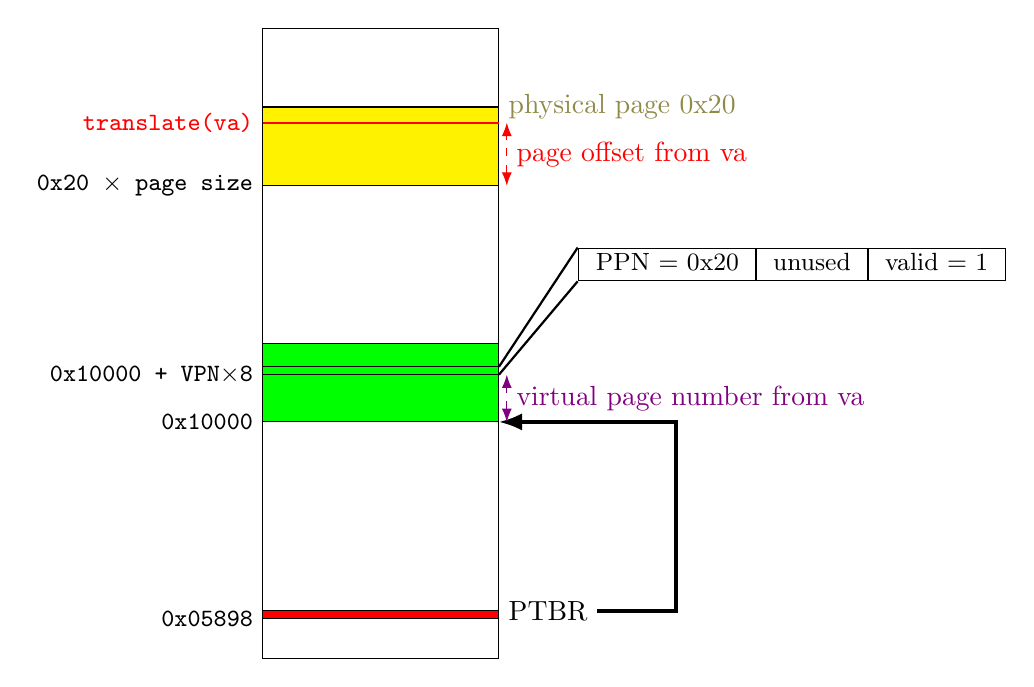
\begin{tikzpicture}
\draw (0, 0) rectangle (3, -8);
\draw[fill=red] (0, -7.5) rectangle (3, -7.4)
    node[right] (ptbr) {PTBR};
\draw[fill=green] (0, -4) rectangle (3, -5);
\draw[-Latex, very thick] (ptbr.east) -- ++(1cm, 0cm) |- (3, -5);
\node[font=\small\tt,anchor=east] at (0, -7.5) {0x05898};
\node[font=\small\tt,anchor=east] at (0, -5) {0x10000};
\node[font=\small\tt,anchor=east] at (0, -4.4) {0x10000 + VPN$\times$8};
\node[font=\small\tt,anchor=east] at (0, -2) {0x20 $\times$ page size};

\draw[Latex-Latex,violet,dashed] (3.1, -5) -- (3.1, -4.4) node[midway,right] {virtual page number from va};
\draw (0, -4.4) rectangle (3, -4.3);
\node[anchor=west,font=\small,inner sep=0mm] (pte) at (4, -3) {
    \begin{tabular}{|l|l|l|} \hline
    PPN = 0x20 & unused & valid = 1 \\ \hline
    \end{tabular}
};
\draw[thick] (3, -4.4) -- (pte.south west);
\draw[thick] (3, -4.3) -- (pte.north west);

\draw[fill=yellow] (0, -2) rectangle (3, -1)
    node[right,yellow!50!black] {physical page 0x20};
\draw[Latex-Latex,red,dashed] (3.1, -2) -- (3.1, -1.2) node[midway, right] {page offset from va};
\draw[thick,red] (0, -1.2) -- (3, -1.2);

\node[red,font=\small\tt,anchor=east] at (0, -1.2) {translate(va)};

\end{tikzpicture}
\end{frame}

\begin{frame}[plain]{first allocate\_page(va) [LEVELS=1]}
\begin{tikzpicture}
\draw (0, 0) rectangle (3, -8);
\draw[fill=red] (0, -7.5) rectangle (3, -7.4)
    node[right] (ptbr) {PTBR};
\begin{visibleenv}<2->
\draw[fill=green] (0, -4) rectangle (3, -5);
\draw[alt=<2>{red},-Latex, very thick] (ptbr.east) -- ++(1cm, 0cm) |- (3, -5);
\end{visibleenv}
\node[font=\small\tt,anchor=east] at (0, -7.5) {0x05898};
\begin{visibleenv}<2->
\node[font=\small\tt,anchor=east] at (0, -5) {NEW0};
\node[font=\small\tt,anchor=east] at (0, -4.4) {NEW0 + VPN$\times$8};
\end{visibleenv}

\draw[Latex-Latex,violet,dashed] (3.1, -5) -- (3.1, -4.4) node[midway,right] {virtual page number from va};
\draw (0, -4.4) rectangle (3, -4.3);
\begin{visibleenv}<2>
\node[anchor=west,font=\small,inner sep=0mm] (pte) at (4, -3) {
    \begin{tabular}{|l|l|l|} \hline
    unused & unused & \myemph<2>{valid = 0} \\ \hline
    \end{tabular}
};
\end{visibleenv}
\begin{visibleenv}<3->
\node[draw=red,anchor=west,font=\small,inner sep=0mm] (pte up) at (4, -3) {
    \begin{tabular}{|l|l|l|} \hline
    PPN = \myemph{NEW1} & unused & \myemph<2>{valid = 1} \\ \hline
    \end{tabular}
};
\end{visibleenv}
\draw[thick] (3, -4.4) -- (pte.south west);
\draw[thick] (3, -4.3) -- (pte.north west);

\begin{visibleenv}<3->
\draw[fill=yellow] (0, -2) rectangle (3, -1);
\node[font=\small\tt,anchor=east] at (0, -2) {\myemph{NEW1} $\times$ page size};
\draw[decorate,decoration={brace,mirror}] (3.1, -2) -- (3.1, -1) node[midway,right] {from posix\_memalign};
\end{visibleenv}
\end{tikzpicture}
\end{frame}

\begin{frame}[plain]{allocate\_page(va) [LEVELS=1]}
\begin{tikzpicture}
\draw (0, 0) rectangle (3, -8);
\draw[fill=red] (0, -7.5) rectangle (3, -7.4)
    node[right] (ptbr) {PTBR};
\draw[fill=green] (0, -4) rectangle (3, -5);
\draw[-Latex, very thick] (ptbr.east) -- ++(1cm, 0cm) |- (3, -5);
\node[font=\small\tt,anchor=east] at (0, -7.5) {0x05898};
\node[font=\small\tt,anchor=east] at (0, -5) {0x10000};
\node[font=\small\tt,anchor=east] at (0, -4.4) {0x10000 + VPN$\times$8};

\draw[Latex-Latex,violet,dashed] (3.1, -5) -- (3.1, -4.4) node[midway,right] {virtual page number from va};
\draw (0, -4.4) rectangle (3, -4.3);
\begin{visibleenv}<1>
\node[anchor=west,font=\small,inner sep=0mm] (pte) at (4, -3) {
    \begin{tabular}{|l|l|l|} \hline
    unused & unused & \myemph<2>{valid = 0} \\ \hline
    \end{tabular}
};
\end{visibleenv}
\begin{visibleenv}<2>
\node[draw=red,anchor=west,font=\small,inner sep=0mm] (pte up) at (4, -3) {
    \begin{tabular}{|l|l|l|} \hline
    PPN = \myemph{NEW} & unused & \myemph<2>{valid = 1} \\ \hline
    \end{tabular}
};
\end{visibleenv}
\draw[thick] (3, -4.4) -- (pte.south west);
\draw[thick] (3, -4.3) -- (pte.north west);

\begin{visibleenv}<2->
\draw[fill=yellow] (0, -2) rectangle (3, -1);
\node[font=\small\tt,anchor=east] at (0, -2) {\myemph{NEW} $\times$ page size};
\draw[decorate,decoration={brace,mirror}] (3.1, -2) -- (3.1, -1) node[midway,right] {from posix\_memalign};
\end{visibleenv}

\end{tikzpicture}
\end{frame}
